%!TEX root = ../dokumentation.tex

\chapter{Planung und Konzeption}
In diesem Kapitel werden die Anforderungen für ein digitales Funkübertragungssystem definiert, welches die Möglichkeit bieten soll beliebige Signale im Bereich der Dezimeterwelle zu analysieren und zu verarbeiten. Das aus dieser Definition resultierende System wird im Verlauf dieses Kapitels geplant und implementiert.\\
Um möglichst viele Dienste im Frequenzbereich der Dezimeterwelle analysieren zu können sollte der Hardwareaufbau, bestehend aus Antenne und digitalem Empfängersystem, folgende Eigenschaften besitzen:
\begin{itemize}
	\item Die Antenne sollte möglichst breitbandig sein. Sie muss mindestens den vorgegeben Bereich zwischen 300 MHz und 3000 MHz abdecken.
	\item Um ein Signal vollständig zu erfassen muss auch das digitale Empfängersystem eine ausreichende Kanalbandbreite aufweisen.
	\item Die Abtastrate des Systems muss gemäß Abschnitt \ref{abtasttheorem} ausreichend hoch sein um das Signal rekonstruieren zu können.
	\item Das Das System muss mit einem Unix-ähnlichem Betriebssystem oder mit Microsoft Windows bedienbar sein.
\end{itemize}%TODO: Gibt es noch mehr Anforderungen? Kosten, etc?

Die aufgeführten Anforderungen werden bei der Planung des Systems, besonders bei der Auswahl der Hardware, berücksichtigt. 

\section{Aufbau/Entwurf}
%TODO
\section{SDR Sharp}
SDR\# (gesprochen: \enquote{SDR Sharp}) ist eine kostenlose Software von Airspy \cite{airspy:2018}, die ausschließlich für Microsoft Windows erhältlich ist. Mit dieser Anwendung lassen sich u. a. mittels Software Defined Radio Systemen empfangene Signale auslesen und etwa im Frequenzbereich oder in einem Wasserfalldiagramm visualisieren.
So lassen sich einige Modulationsarten relativ schnell und rein visuell identifizieren.
%TODO Bild von SDR# hinzufügen: Am besten ein FM Radiosignal, und erklären woran man die FM Modulation erkennt.


\section{GNU Radio}
GNU Radio \cite{gnuradio} ist ein freies, quelloffenes Entwicklerwerkzeug zur Implementierung von Software Defined Radio mittels Signalverarbeitungsblöcken. Es kann mit externer Funkhardware oder als Simulation ohne zusätzliche Hardware genutzt werden. GNU Radio ist im Hobbybereich weit verbreitet, wird aber auch in der Wissenschaft und im kommerziellen Bereich genutzt. GNU Radio Programme können zusätzlich durch selbst programmierte Ergänzungsblöcke erweitert werden. Die können wahlweise in den Programmiersprachen Python oder C++ geschrieben werden, wobei sich besonders für echtzeitkritische Signalverarbeitungen letzteres anbietet.\\
GNU Radio bietet zusätzlich eine grafische Oberfläche mit \ac{GRC}, die es ermöglicht Blockschaltbilder als Flowgraph darzustellen.
%TODO Bild von GNU Radio hinzufügen

\subsection{Funktionsweise}
GNU Radio verarbeitet den Datenstrom, der vom Empfänger kommt, oder bereitet Daten vor, um diese zu senden. Dabei ist die gesamte Datenverarbeitung in Blöcke eingeteilt, die  beliebig  zusammengestellt  werden können. GNU Radio liefert eine Vielzahl von Filtern, Kanal-Codes, Synchronisationselementen, Equalizern, Demodulatoren, und weitere gängige Werkzeuge der Nachrichten- und Funktechnik. Diese Blöcke stellen die Hardwarekomponenten klassischer Funkhardware dar. Falls nötig können auch selbst Blöcke hinzugefügt werden. Dabei sollte darauf geachtet werden, dass ein Block genau eine Aufgabe erledigt, damit er so vielseitig wie möglich eingesetzt werden kann. GNU Radio bietet die Möglichkeit, diese Blöcke miteinander zu verbinden und regelt dadurch den Datenfluss zwischen verbundenen Blöcken. \\
Für die digitale Verarbeitung von Daten kommen in GNU Radio verschiedene Datentypen zum Einsatz: Der Datenstrom des Empfängers besteht in den meisten Fällen aus komplexen Zahlen, also einem Datentyp, bei dem jedes Datum aus zwei Float-Werten, dem Imaginärteil und dem Realteil, besteht (siehe Abschnitt \ref{iq}). \\
Als Ein- oder Ausgänge eines Blocks können jedoch verschiedene Datentypen zum Einsatz kommen, üblicherweise Short, Byte, Integer und Float. Der Datentyp am Eingang und Ausgang eines Blockes muss dabei nicht gleich sein.\\
Um mit GNU Radio eine SDR-Anwendung zu erstellen, muss man Blöcke, die die einzelnen Funktionseinheiten darstellen, miteinander zu einem Graphen kombinieren. Sollte ein benötigter Block nicht verfügbar sein, kann man diesen mittels einem Tool selbst hinzufügen. Beim Starten des Graphen ruft GNU Radio nun jeden Block nacheinander auf und stellt sicher, dass Daten von einem Block zum Nächsten weitergereicht werden. Ergebnisse  können  durch  Graphical  User  Interface  (GUI)-Blöcke dargestellt werden. Diese nutzen die freien und plattformübergreifenden GUI-Toolkits.


\section{Hardware}
\subsection{Antenne} %TODO: Sollen wir eine von den Antennen, die wir uns anfangs auchgesucht haben mit unserer vergleichen und eine Entscheidungsmatrix aufstellen?  SO dass man sieht, dass wir uns Alternativen angeschaut haben?
Eine Antenne die aus der Aufgabenstellung hervorgeht, muss dementsprechend den Frequenzbereich der Dezimeterwelle abdecken. 
Grundsätzlich gibt es zwei Möglichkeiten ein solches Analysesystem zu betreiben: Mit stationärer oder mobiler Antenne. Letzteres bietet die Möglichkeit das Gerät auch unterwegs nutzen. 
Aus Gründen wie Flexibilität und Mobilität entschieden wir uns jedoch dagegen. Eine mobile Antenne, die den Frequenzbereich der Dezimeterwelle abdecken, würde relativ groß und ziemlich teuer sein. Deshalb haben wir uns auf eine stationäre Antenne geeinigt, da diese preislich als auch dem Verwendungszweck dennoch am nächsten kommt. Wir haben uns für die  Sirio SD 3000N entschieden, ihr preis liegt bei 90 Euro und deckt den kompletten Frquenzbereich der Dezimeterwelle ab.\newline %TODO: "wir", "uns" streichen
%TODO: Was sind genau die Vorteile unserer Antenne? -> Aufzählen

\begin{figure}[ht]
	\centering
	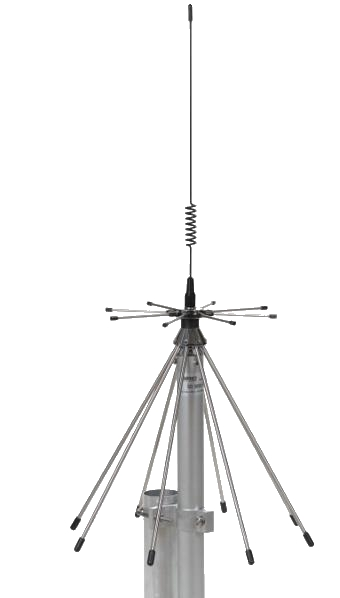
\includegraphics[width=0.4\textwidth]{SirioSD3000N.png} %TODO: Antenne bzw. Bestandteile beschriften? 
	\caption[Sirio SD 3000N stationäre Funkantenne]{Sirio SD 3000N stationäre Funkantenne. Quelle: \cite{Funktechnik:2018}} 
	\label{Sirio SD 3000N Antenne}
\end{figure}

Aufgrund analytischen Zwecken haben werden zwei Antennen für die Aufgabe erworben, somit können wir an zwei unterschiedlichen Standorten eine Analyse der Metainformationen betrachten. %TODO: Neu schreiben. Das ist ziemlich wirr :D


\begin{table}[ht]
	\centering
\begin{tabular}{c|c}
	Modell & Sirio SD 3000N \\
	\hline
	Antennentyp & Discone Antenne \\ 
	\hline 
	Bandbreite & 300 MHz - 3 GHz \\ 
	\hline 
	Länge &  \\ 
	\hline 
	Preis in \euro &  \\ 
	\hline 
	Installationsart & Stationär \\ 

\end{tabular} 
	\caption{Produktinformationen der Sirio SD 3000N Antenne}
\end{table}


%TODO: Präsentation vom Hochfrequenztechnik aus Mechtronik siehe WhatsApp

\subsection{SDR-Gerät} %TODO: Struktur in den Text bringen. Absätze, Aufzählungen, etc
Ein Software Defined Radio Gerät, das man experimentell betreiben kann, reicht von mehreren tausend Euro teuren Forschungsgeräte bis zu kostenlosen Geräten, da selbst mittels einem Mikrofoneingang der Soundkarte am Computers, manche Signale empfangen werden können. Die Geräte unterscheiden sich hauptsächlich im Frequenzbereich, der maximalen Bandbreite und der Abtastrate. \\
Beim Computer kommen häufig Universal Serial Bus (USB), Ethernet als Schnittstelle zum  Einsatz.
Da theoretisch nur Signale empfangen werden sollen, würde ein DVB-T-Stick eine günstige Option darstellen. Mithilfe eines entsprechenden Treibers kann der Stick mit GNU Radio genutzt werden, jedoch deckt sich der Frequenzbereich des Gerätes nicht, mit dem innerhalb der Aufgabenstellung der Dezimeterwelle.


Das SDR-Gerät muss in Kombination mit der Funkantenne über den kompletten Funkbereich der Dezimeterwelle erstrecken, um die Metainformationen in diesem Bereich zu analysieren. Aus diesem Grund kann ein solchen Gerät für diese Arbeit nicht verwendet werden.
Ein gutes Preis-Leistungsverhältnis bietet das HackRF One Board \cite{greatscott}. Die HackRF One Platine ist ein flexibles Testmodul für die Funkmesstechnik, das wie ein Software Defined Radio (SDR) arbeitet. Sie ist ein Open Source Hardware Transceiver, der hauptsächlich zu eigenen Versuchen und Messungen für SDRs eignet, außerdem ist dieses Gerät für die HF-Technik und messtechnischen Versuchsaufbauten im Amateurfunk vergleichsweise geringen Preises von rund 300 Euro sehr beliebt.
Der Hack RF One deckt einen weiten Frequenzbereich von 1 bis 6000 MHz (6 GHz) ab, und erfasst damit sehr viele Frequenzbänder für kommerzielle, experimentelle und Amateurfunk-Anwendungen. Die Hardware bietet eine maximale Abtastrate des Signales von 20MS/s, dadurch werden Messungen und Experimente auch mit breitbandigen Signalen wie DECT, WFM oder WLAN möglich, jedoch nur halbduplex. Der AD-Wandler arbeitet mit 8 Bit Datenbreite und erreicht somit einen theoretischen Dynamikbereich von 48dB. Die digitalisierten I/Q Daten werden auf einem nachgeschalteten CPLD weiterverarbeitet und über den integrierten ARM-Prozessor per USB ausgegeben. Die gesamte Schaltung des HackRF Boards ist sehr stromsparend ausgelegt, sie wird komplett über USB versorgt. Die Platine hat eine Mikro-B USB Buchse. Abschließend lässt sich sagen, dass die oben genannten Gründe für eine Nutzung dieses Gerätes sprechen \cite{wimo:2018}.


\begin{figure}[ht]
	\centering
	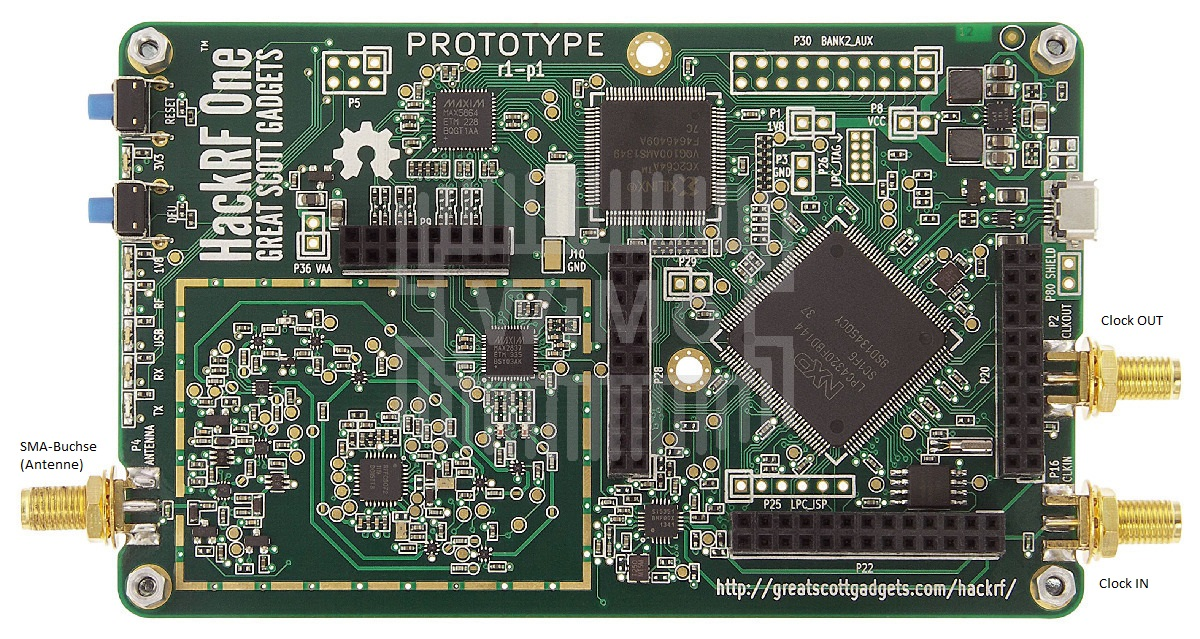
\includegraphics[width=0.75\textwidth]{HackRFOne.png}
	\caption[Hack RF ONE Platine]{Hack RF ONE Platine. Quelle: \cite{HackRFOne:2018}} 
	\label{HackRFOne}
\end{figure}


\begin{table}[ht]
	\centering
	\begin{tabular}{c|c}
		Modellbezeichnung & HackRF One \\
		\hline
		Hersteller & Great Scott Gadgets\\ 
		\hline 
		Bandbreite & 20 MHz \\ 
		\hline 
		Abtastrate & \( 20 \times 10^{6} \) Hz \\ 
		\hline 
		Preis in \euro &  \\ 
		\hline 
		Installationsart & Mobil \\ 
		
	\end{tabular} 
	\caption{Produktinformationen des HackRF One}
\end{table}


\begin{figure}[ht]
	\centering
	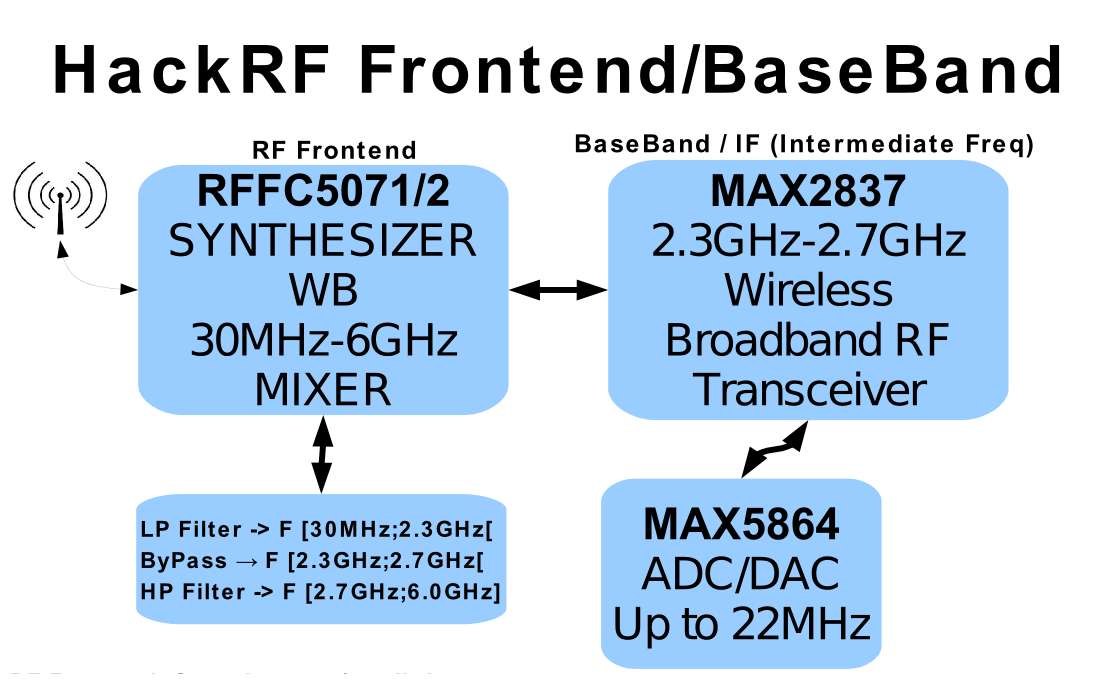
\includegraphics[width=0.7\textwidth]{hackrf-blockdiagram-frontend-baseband.png}
	\caption[Hack RF One Frontend/Baseband]{Hack RF One Frontend/Baseband. Quelle: \cite{hackrf-wiki:2016}} 
	\label{HackRFOne-Blockschaltbild}
\end{figure}
